%********VORAUSSETZUNGEN & GRUNDLAGEN*********
\chapter{Fundumentals}
\label{sec:Fundumentals}
\section{STM-Imaging}
The Scanning Tunneling Microscope was introduced in 1981 by Gerd Binning and Heinrich Roherer. 
With this measuring technique it is possible to resolve a conductive surface with a precission beyond that of conventional light based Microscopes.
In contrast to other electron based microscopy like Scanning Electron Microscopes (SEM) it uses the quantum mechanical phenomenon of tunneling.
In classical mechanics, objects cannot overcome a potential if their energy $E < V_0$, as observed in gravitational interactions.
This phenomenon is observed for quantum mechanical particles like electrons, which can surpass a potential barrier despite the initial expectation that they should not be able to.
The STM uses this effect by precisely positioning a sharp conductive tip close to the surface and applying a bias voltage.
Most STM are operated in Ultra-High-Vacuum (UHV), where the distance between the tip and the surface represents the tunneling barrier.
By varying the bias voltage, the tunneling probability can be changed, thereby affecting the tunneling current.
If the bias voltage, also referred to as the potential difference, is kept constant, the tunneling current is primarily dependent on the distance between tip and surface.
The tip is moved in the x-,y-plane where a grid is established. 
There are two modes of operation, the constant-height and the constant-current mode.
The latter is especially useful for irregular surfaces, because the tip is moved up and down to keep the tunneling current constant.
The movement signal of the piezos is then converted into height.
In constant-height mode the position of the tip stayes fixed and the tunneling current $I_t$ is measured and converted into height information. \\

\newpage
\begin{wrapfigure}{r}{0.5\textwidth}
    \centering
    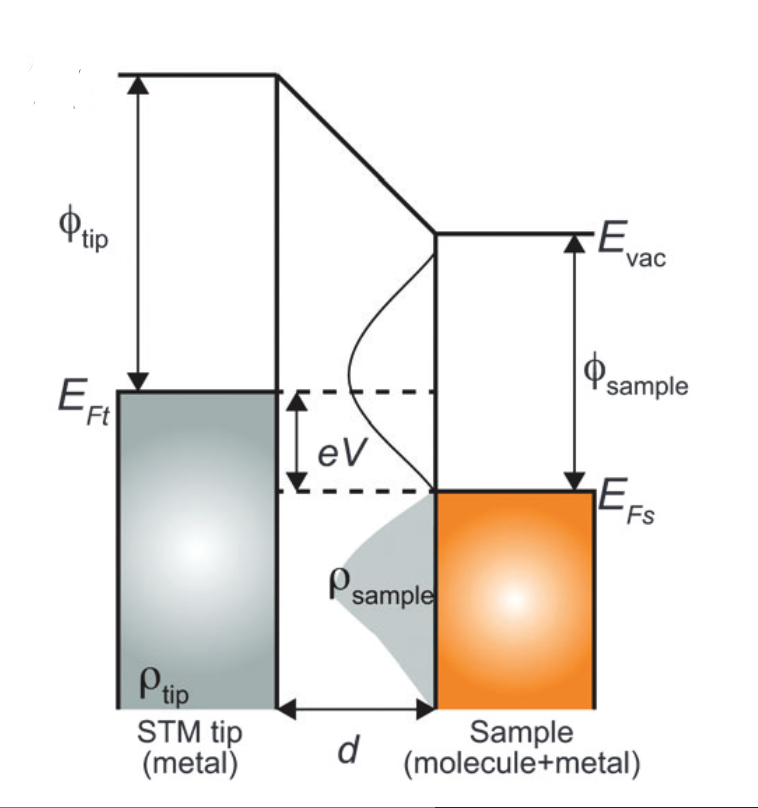
\includegraphics[width=0.4\textwidth]{graphics/Tunneling_diagram_japan.PNG}
    \caption{Energy diagram of the tunneling  junction with a positive bias voltage applied. $\Phi_{tip}$ \& $\Phi_{sample}$: working functions of either tip and sample, $E_{vac}$: vacuum energy level,  $E_{ft}$ \& $E_{fs}$: Fermi Energys of the tip and sample,  $\rho_{tip}$ \& $\rho_{sample}$: density of states of tip and sample,  $eV$: potential difference caused by applying a bias Voltage $V$ (picture source: \cite{Kano}) }
    \label{fig:energy_diagram}
\end{wrapfigure}

The tunneling current, at a arbituery gridpoint, is influenced by the electronic structure of the tip and sample.
If the tip is in vicinity of the metallic substrate the fermi energies align, resulting in an equal probability of electrons tunneling from the tip to the sample and vice versa.
This consequently results in a zero net current. 
Through the introduction of a electric potential $V_{bias}$ the fermi energies of tip and sample can be shifted relative to each other (Figure \ref{fig:energy_diagram}).
If the bias voltage is positive the fermi energy of the sample is pushed down and electrons from occupied states in the tip can tunnel into the empty states of the sample.
Consequently if the bias voltage is negative electrons from the filled states of the sample tunnel into the tip.
The tunneling current is influenced by the distance $d$ between orbitals of the tip and the sample, which makes it possible to gain information about the electronic structure of the sample.
This is not really a representation of the real structure of the atoms or molecules, but the Local Density of States (LDOS) of the sample´s surface.
Utilizing this in Scanning Tunneling Spectroscopy (STS) provides additional information beyond the sample's topography.
Such as the chemical composition, bonding, the energy gap and band-bending effects [\cite{cbai}].
\newpage
\section{Mathematical Foundation STM}

To understand the tip sample interaction one must look at the quantum-mechnical Foundation behind it.
At its simplest the tip can be approximated as spherical potential well (Figure \ref{fig:tip_scheme}). $R$ is in that case the radius of the tip located at position $\vec{r_0}$ with the distance $d$ from the surface.
First order pertubation theory gives the following expression (Eq. \ref{eq:tunneling_pert}) for the tunneling current of this system [\cite{PhysRevLett}]:
\begin{equation}
    I = \frac{2 \pi e}{\hbar} \sum_{\mu \nu} f(E_{\mu})[1 - f(E_{\nu}+eV_{bias})]\cdot |M_{\mu \nu}|^2 \delta(E_{\mu}- E_{\nu})
    \label{eq:tunneling_pert}
\end{equation}\\

\begin{wrapfigure}{r}{0.3\textwidth}
    \centering
    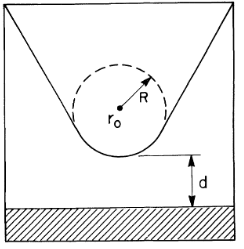
\includegraphics[width=0.3\textwidth]{graphics/fundamental_tip_sheme.PNG}
    \caption{Schematic depiction of the tip geometry [\cite{PhysRevLett}]}
    \label{fig:tip_scheme}
\end{wrapfigure}

\noindent The fermi distribution $f(E)= (\exp((E-E_F)/k_b T)+1)^{-1}$ gives the ocupation probability of a fermion (electrons) with the Energy $E$ near the fermi level.
In this case it is the ocupation probability of the tip states (denoted by the subindex $\mu$) and the ocupation probability of the sample states ( denoted by the subindex $\nu$).
The tunneling matrix $M_{\mu \nu}$ is related to the derivatives of the sample wave functions $\psi_{\nu} $ at the nucleus of the apex atom [\cite{tunnelmatrix}].
Because the STM Imaging is done at low temperatures and with small voltages the Equation \ref{eq:tunneling_pert} can be simplified to:
\begin{equation}
    I = \frac{2 \pi}{\hbar} e^2 V_{bias} \sum_{\mu \nu}  |M_{\mu \nu}|^2 \delta(E{\nu}-E_F) \delta(E_{\mu}- E_{F})
    \label{eq:tunneling_pert_simple}
\end{equation}
With the tunneling matrix $M_{\mu \nu}$ , which relates to the probability of an electron transitioning from state $\mu$ to state $\nu$ [\cite{tunnelmatrix}]: 
\begin{equation}
    M_{\mu \nu} = \frac{\hbar^2}{2m} \int (\psi_{\mu}^{*} \vec{\nabla} \psi_{\nu} - \psi_{\nu} \vec{\nabla} \psi_{\mu}^{*}) \, d\vec{S}
    \label{eq:tunnelin_matrix}
\end{equation}
To obtain a solution  , the tip wave function can be explicitly chosen as an s-type orbital, this holds true for a tungsten tip as it has a only a s-type orbital occupied in its valence shell.
This orbital has a spherical form [\cite{PhysRevLett}]:
\begin{equation}
    \psi_{\mu} = \Omega_t^{-1/2} * c_t k R e^{kR} ( k|\vec{r}- \vec{r_0}|)^{-1} e^{-k|\vec{r}- \vec{r_0}|}
    \label{eq:tip_wave}
\end{equation}
$\Omega_t^{-1/2}$ is the volume of the probe, $k = \hbar^{-1} \sqrt{2m\phi}$ is the inverse dacay length for the wave functions in vacuum, $c_t$ is a geometry specific constant on the order of 1 and $R$ is the radius of curvuture.
The surface wavefunctions can be approximated as blochwaves, which are plane waves modulated by a periodic function.
In the region of neglible Potential the surface wavefunction can be written as:
\begin{equation}
    \psi_{\nu} = \Omega_{s}^{-1/2} \sum_{G} a_G \exp(- (k^2 + |\vec{k}_{||} + \vec{G}|^2)^{1/2} z)\cdot \exp(i(\vec{k}_{||} + \vec{G})\cdot \vec{x})
    \label{eq:surface_wave}
\end{equation}
Here $\Omega_{s}^{-1/2}$ is the sample volume, $k$ the previously mentioned inverse decay length, $\vec{k}_{||}$ is the surface bloch wave vector and $\vec{G}$ represents the reciprocal surface vector.
Substituting into \ref{eq:tunneling_pert_simple} as seen in executed in [\cite{PhysRevLett}] gives the result:
\begin{equation}
    I = 32 \pi^3e^2 V_{bias}\phi^2 D_t(E_F)R^2 k^{-4} e^{2kR} \cdot \sum_{\nu} |\psi_{\nu}(\vec{r_0})|^2 \delta(E_{\nu} - E_F) 
\end{equation}
Where $D_t(E_F)$ is the Density of States of the Tip at the Fermi Level. 
The sum over the local states of the surface $\psi_{\nu}$ at the Fermi Level ($\delta(E_{\nu} - E_F)$) can be interpreted as the Local Density of States (LDOS).
Using the surface wavefunction one can see that the tunneling current is following an exponential decay, that is proportional to the distance $d$ between the tip and the sample:
\begin{equation}
    I \varpropto e^{-2 \cdot d \sqrt{\frac{2m \phi}{\hbar^2}}}
    \label{eq:propcurrent}
\end{equation}




\newpage

\section{Low Energy Electrons Diffraction (LEED)}
A well collimated beam of electrons with the same wavelengh is directed at a flat surface.
In this case the wavelengh of the incoming electrons is determened by the electric field $U_a$ that acts upon them \ref{eq:electron_wavelengh}.
To see diffraction the wavelengh of the electrons must be in the range of the lattice constant, as is effectively show by the concept of the ewald sphere.
Typically the kinetic energy of the electrons is up to $E_{kin} = e U_a = 200$ eV.
\begin{equation}
    \lambda = \frac{h}{\sqrt{2 m_e e U_a}}
    \label{eq:electron_wavelengh}
\end{equation} 
If the surface is periodic this results in a sharp pattern of spots that reflects the k-space of the crystal.

\begin{wrapfigure}{r}{0.6\textwidth}
    \centering
    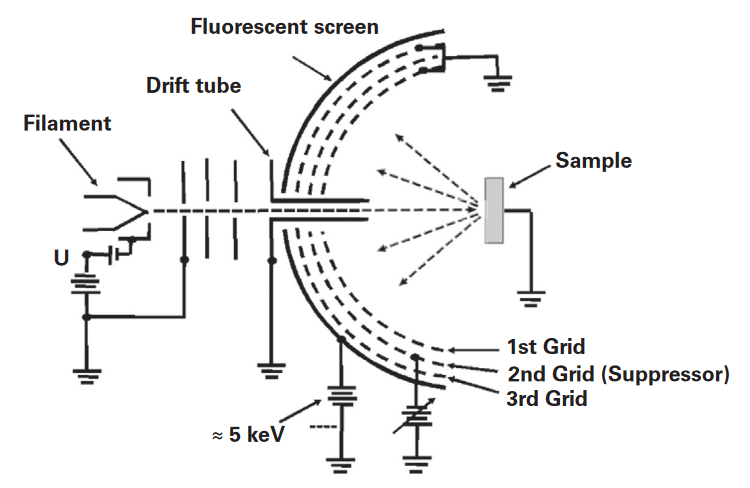
\includegraphics[width=0.5\textwidth]{graphics/fundamental_leed_setup.PNG}
    \caption{A basic three-grid LEED system which utilizes a flourenscent screen as imaging tool \cite{MoritzWolfgang2022SSDb}}
    \label{fig:LEED_Shematics}
\end{wrapfigure}

\noindent The LEED setup consists of a filament which emitts electrons by applying a current.
This electrons are then accelerated and collimated in a drift tube which points at the sample.
Due to interactions of the electrons with the crystal atoms some of them are not diffracted elastically.
To ensure that only the elastically scattered electrons are show on the flourencent screen, a grid system is installed in front of the screen.
The first grid and the sample are both grounded to ensure that the diffracted alectrons propagate undesturbed through the space between the sample and the grid.
A filter Voltage is aplied between the second and third grid that is just below the acceleration voltage.
Electrons which are not elastically scattered are completely stopped, which makes it effectivelly a high pass filter. [\cite{MoritzWolfgang2022SSDb}] \\

\noindent The collimated beam can be represented as a planar wave $e^{i \vec{k_0} \vec{r}}$  outside the surface.
The wavevector $\vec{k_0}$ points in the propagation direction and represents the spacial frequency of the wave.
This vector can be modeled as:
\begin{align}
    |\vec{k_0}| &= \frac{2 \pi}{\lambda} = \frac{\sqrt{2 m_e E}}{\hbar} \\
    \hspace{1cm} \notag \\
    \vec{k_0} &= \begin{pmatrix}
        |k_0|\cos(\varphi)\sin(\vartheta)\\|k_0|\sin(\vartheta)\sin(\vartheta)\\|k_0| \cos(\vartheta)
    \end{pmatrix}
\end{align}
A 2D periodic surfuce structure with a reciprocal basis ($b_1$,$b_2$) causes the plane waves to diffract.
The diffracted waves have the shape $A_g e^{i \vec{k_g} \vec{r}}$ with wave vectors $|\vec{k_g}| = |\vec{k_0}|$.
$\vec{k_g}$ transforms according to $\vec{k_g} = \vec{k_0} + \vec{g}$. 
The reciprocal lattice vector $\vec{g} = 2 \pi ( h b_1 + k b_2)$ represents the individual points where constructive interference is present.
Usually the indices h and k are intergers which characterize the beam, for example (0,0) or (1,1).
It can be shown that the wave vector in vacuum outside the surface is [\cite{MoritzWolfgang2022SSDb}]:
\begin{equation}
    k_g = - \sqrt{\frac{2 m_e E}{\hbar^2} - (k_{0x}+ g_{x})^2 - (k_{0y}+ g_{y})^2}
\end{equation}

%\polyfig{graphics/fundamental_kspace.PNG}{hllohi}{fig:kspace}{graphics/fundamental_kspace_theta.PNG}{fig:kspace_}{helo}

%\begin{figure}[H]
%    \centering
%    \begin{minipage}[b]{0.49\textwidth}
%        \centering
%        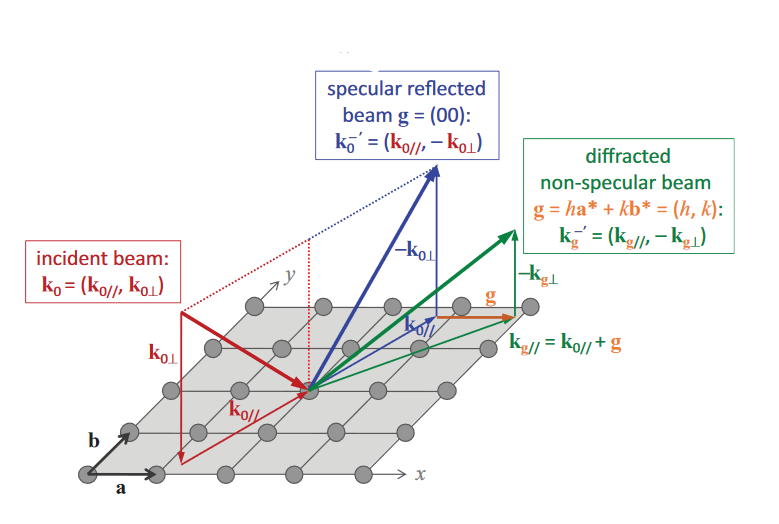
\includegraphics[width=\textwidth]{graphics/fundamental_kspace.PNG}
%        \caption{
%            2D lattice with the reciprocal lattice vectors $\vec{a}$ and $\vec{b}$. 
%            $\vec{k_0}$ (red): incident beam,
%            $\vec{k_{0}^{-}}'$ (blue): specular reflected beam,
%            $\vec{k_{g}^{-}}'$ (green): non-specular diffracted beam, }
%        \label{fig:kspace}
%    \end{minipage}
%    \begin{minipage}[b]{0.49\textwidth}
%        \centering
%        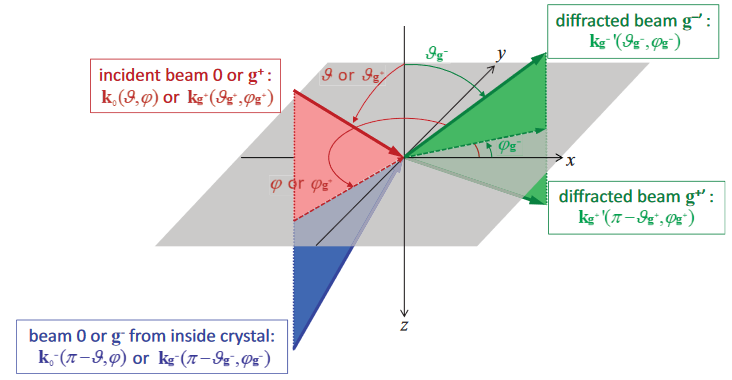
\includegraphics[width=\textwidth]{graphics/fundamental_kspace_theta.PNG}
%        
%        \caption{hgh}
%        \label{fig:kspace2}
%    \end{minipage}
%\end{figure}
%

\duofigcom{graphics/fundamental_kspace.PNG}{fig:kspace}{graphics/fundamental_kspace_theta.PNG}{fig:kspace2}{
    (a): 2D lattice with the reciprocal lattice vectors $\vec{a}$ and $\vec{b}$. 
    $\vec{k_0}$ (red): incident beam,
    $\vec{k_{0}^{-}}'$ (blue): specular reflected beam,
    $\vec{k_{g}^{-}}'$ (green): non-specular diffracted beam, }{}




\section{Adsoption}
\newpage